\documentclass[12pt,letterpaper]{article}
\usepackage{geometry}
\geometry{margin=1in}
\usepackage{graphicx}
\usepackage{float}

\setlength{\parindent}{0pt}
\setlength{\parskip}{0.5em}

%make lists tighter
\usepackage{enumitem}
\setlist{nolistsep}

%reduce spacing before and after section
\usepackage{titlesec}
% reduce section, subsection, etc spacing
\usepackage{titlesec}
\usepackage{amsmath, amssymb}
\titlespacing*{\section}{0pt}{0\baselineskip}{0\baselineskip}
\titlespacing*{\subsection}{0pt}{0\baselineskip}{0\baselineskip}
\titlespacing*{\subsubsection}{0pt}{0\baselineskip}{0\baselineskip}

%reduce list spacing
\usepackage{enumitem}
\setlist{nosep}

\usepackage[hidelinks]{hyperref}

\title{Lab 3.1 - FMRI, Stat 214, Spring 2025\vspace{-2em}}

% submission must not contain any of your names
% but feel free to make a version for yourself with your names on it
% \author{Your names}

\begin{document}
\maketitle


\section{Introduction}

There is a need to understand how a human brain interprets language. Functional Magnetic Resonance Imaging (fMRI) allows researchers to observe how the brain responds to language stimuli by measuring blood-oxygen level-dependent (BOLD) signals across different brain regions. This report builds on prior work by Jain and Huth (2018), who demonstrated that introducing context into word representations significantly improves the ability to model fMRI responses. 

 Particularly, we explore how different word embedding strategies affect the prediction of whole-brain BOLD responses during natural story listening. We evaluate three types of embeddings: Bag-of-Words, Word2Vec, and GloVe. For each embedding type, we construct time-aligned feature matrices, downsample them to match fMRI scan rates, and apply a ridge regression model to predict voxel-wise responses.  To capture the temporal dynamics of neural processing, we also use lagged features. Finally, we compare the performance of the different models using correlation-based evaluation metrics across two subjects. 

Our goal is to assess which embedding methods most effectively explain brain activity, and whether richer semantic and contextual information improves predictive performance over simpler models.


\section{Exploratory Data Analysis}



This section describes the structure and characteristics of the data used in our analysis. 

There are two types of data: whole-brain blood-oxygen level-dependent (BOLD) signals measured at various points across the podcast scanned by fMRI ( treated as “response”), and the raw text for the stories (treated as “stimulus”).


The response data was collected from two anonymized subjects, “subject 2” and “subject 3,” who were scanned using fMRI while listening to the same set of 101 stories. Each fMRI scan collected the signals from 94,251 voxels for subject 2 and 95,556 voxels for subject 3, which suggests individual differences in brain structure and size. Due to this variability, it is not feasible to train a model on one subject's data and apply it directly to predict another. Hence, we decided to randomly split the data into 101 stories, using 68 stories (about 70\%) as the training data and 33 stories (about 30\%) as the test data, train the model, and make the prediction for each subject. 


The stimulus data includes the text data that has been segmented into words and the time data for when each word was played. Once word embeddings are generated from the text, these timestamps allow us to align each word with the corresponding fMRI scan time point, allowing the dimensions of the response and stimulus data to be matched.

To better understand the dataset, we performed some exploratory data analysis. For each story in the training data, the minimum and maximum word counts ranged from 697 and 3,274 respectively, while the minimum and maximum unique word counts ranged from 278 and 1,052 respectively. When the training data was totaled, there were 10,356 unique words. As discussed in the following sections, the fact of having more than 10,000 unique words leads to stimulus $X$ becoming very large and that can make ridge regression computationally expensive without appropriate dimensionality reduction strategies.


\section{Embeddings}
\subsection{Generate embedding vectors via bag-of-words}
We begin by constructing an embedding using the Bag-of-Words approach. The training data contains 10,356 unique words (hereafter referred to as the “word list”). For each word, we create a one-hot vector in $\mathbb{R}^{10356}$, where the position corresponding to the word is set to 1 and all other positions are 0. Concatenating these vectors vertically yields an  $R^{wordcount \times 10356}$ embedding matrix. The column dimensions of the embedding matrices are the same for all stories, which allows all training data to be combined when performing ridge regression to create a single prediction model.

For example, if the 100th word in the word list is "I" and the first word in the story is also "I", the one-hot vector for the first word in the story will be an $R^{10356}$ vector $(0,...,0,1,0,...,0)$ whose 100th element is "1" and otherwise "0". As a result, $(0,...,0,1,0,...,0)$ vector becomes the first row of the embedding matrix.

However, this high-dimensional embedding matrix poses computational challenges. Even after downsampling (as described in the following section), the dimensionality remains too large for efficient ridge regression. Therefore, we constructed a reduced corpus containing the 300 most frequent words in the training data. Each word is now represented by a vector in $\mathbb{R}^{300}$, resulting in a reduced embedding matrix of dimension $\mathbb{R}^{\text{wordcount} \times 300}$. We also chose 300 dimensions to align with the dimensionality of the Word2Vec and GloVe embeddings used later in the analysis, enabling direct and fair comparison across embedding methods.

It is worth noting that the 300-word corpus includes common function words such as “and” and “the,” which make no sense in context implying little semantic meaning. Nevertheless, we decided not to remove these terms from our corpus. This is because, even if these words do not play an important role in the meaning, their impact on BOLD signals is not certain as our scientific interest is limited. In addition, if we remove them and pick up the words used less-frequently, making $X$ too sparse and diminishing model prediction and performance. 

To prevent data leakage, the corpus includes only words observed in the training set, and does not include words that only appear in the test data.

As mentioned earlier, the dimension of the embedding matrix is $R^{wordcount \times 300}$, whose row dimension does not match the number of the fMRI scans. Therefore, in the next section, we need to downsample the embedding matrix to create feature matrices.

\subsection{Downsampling the features}

We will use the provided "downsample\_word\_vectors" function to align the dimension with the number of the fMRI scans. The function uses the Lanczos interpolation to determine the weight of each data point and obtain a weighted sum of the data points to reduce the dimension. This is equivalent to collecting the vectors of words played before and after a fMRI scan to create a new vector in which the words' information is aggregated. As each new vector aggregates the information of the words affecting the brain at the time of the fMRI scan, it will contribute to predicting the BOLD signals.

Mathematically, let $X_{old} \in R^{wordcount \times 300}$ be the original embedding, $X_{new} \in R^{\#\text{fMRI scan} \times 300}$ be the new embedding, $t_{old} \in R^{wordcount}$ be the vector of the time points when each word was played, $t_{new} \in R^{\#\text{fMRI scan}}$ be the vector of the time points after the interpolation, and $w$ be the window of the Lanczos interpolation (here, $w = 3$). The new embedding is defined as:

\begin{align*}
X_{new} &= L(t_{new}, t_{old}, w) X_{old}, \hspace{2mm}\text{where}\hspace{2mm} L(t_{new}, t_{old}, w) \in R^{\#\text{fMRI scan} \times wordcount}
\end{align*}
\begin{align*}
L(t_{new}, t_{old}, w)_{i, j} &= 
\begin{cases}
    1 & \text{, if } \frac{t_{new, i} - t_{old, j}}{2} = 1 \\
    \dfrac{w \cdot sin(\pi\frac{t_{new, i} - t_{old, j}}{2}) \cdot sin(\frac{\pi}{w} \frac{t_{new, i} - t_{old, j}}{2})}{\pi^2 (\frac{t_{new, i} - t_{old, j}}{2})^2} & \text{, if } -w \leq \frac{t_{new, i} - t_{old, j}}{2} \leq w \\
    0 & \text{, otherwise}
\end{cases}
\end{align*}

Lanczos interpolation integrates the data $X$ around each timepoint (each element of $t_{new}$) with different weights based on the distance from the timepoint, to reduce the dimension of $X$ smoothly. As a result, the feature matrix $X_{new}$ aggregates the information of the word played before and after the fMRI scan.

Finally, by deleting the first 5 and last 10 rows of the interpolated feature matrix $X_{new}$, the number of rows of $X_{new}$ matched the number of fMRI scans taken while listening to each story.

\subsection{Lagged versions of the features}
The feature matrix $X_{new}$ created by the previous section aggregates the information of the word played before and after the fMRI scan. In other words, if a certain amount of time passes between the word being played and the fMRI scan, the word information will not be reflected in $X_{new}$. However, we should assume that the subjects retain the information about the words that have been played for a more extended period. Therefore, for each column of $X_{new}$, we created the lagged data with the delay [1, 2, 3, 4]. We decided to construct $X_{new}$ solely by the lag values since the downsampling process caused the data at time $t$ to be mixed with the future information, which the subjects did not listen at that time.

We implemented the code by using the provided "make\_delayed" function. As a result, $X_{new}$ now includes the lagged values of [1, 2, 3, 4], so the column dimension has increased by a factor of four. Therefore, the size of $X_{new}$ becomes $R^{\#\text{fMRI scan} \times 1200}$.

\subsection{Embedding from pretrained models: Word2Vec and GloVe}

In addition to the simple Bag-of-Words representation, we implemented two other embedding methods using pre-trained models: Word2Vec and GloVe (Global Vectors for Word Representation). These methods generate dense, low-dimensional vector representations that capture semantic relationships between words rather than simply recording word occurrences.

\subsubsection { Word2Vec Implementation} 

Word2vec is a neural network-based embedding method for obtaining vector representations of words. These vectors capture information about the meaning of the word based on the surrounding words. This algorithm estimates these representations by modeling text in a large corpus. Once trained, such a model can detect synonymous words or suggest additional words for a partial sentence.

Word2Vec uses two main model architectures: Continuous Bag-of-Words (CBOW) and Skip-gram. In our implementation, we use the Skip-gram model, which predicts the surrounding context words given a target word. This is the reverse of the CBOW approach, which predicts a target word from context words. 

The Skip-gram model performs particularly well with small amounts of training data and is effective at representing rare words or phrases. Mathematically, it works by maximizing the probability of observing context words within a specific window around the current word. Its objective function can be expressed as:

\begin{equation}
J(\theta) = \frac{1}{T} \sum_{t=1}^{T} \sum_{\substack{-c\leq j \leq c \\ j \neq 0}} \log p(w_{t+j}\mid w_t)
\end{equation}

where $T$ is the total number of words, $w_t$ is the target word, and $w_{t+j}$ represents context words within a window. The probability is calculated using softmax: 

\begin{equation}
p(w_O \mid w_I) = \frac{\exp\left({v'_{O}}^\top v_{I}\right)}{\sum_{w=1}^{|V|} \exp\left({v'_{w}}^\top v_{I}\right)}
\end{equation}


where $v_I$ is the input vector and $v'_O$ is the output vector for the words.

For our implementation, we use the pre-trained Word2Vec model from the Google News corpus, which provides 300-dimensional vectors for approximately 3 million words and phrases.

The implementation process involved:

\begin{itemize}[itemsep=0.2cm]
    \item Loading the pre-trained Word2Vec model using the gensim library
    \item Creating embedding matrices for each story where each row corresponds to a word
    \item Mapping each word to its corresponding 300-dimensional vector
    \item Handling words not found in the vocabulary by maintaining zero vectors
\end{itemize}


Unlike Bag-of-Words, which creates sparse one-hot vectors, Word2Vec produces dense vectors that capture semantic similarities between words through the relative positions of words. For example, analogical relationships like "king" is to "queen" as "man" is to "woman" are preserved in the geometric properties of the vectors. Words with similar meanings have vectors that are closer together in the 300-dimensional space. 

\subsubsection {GloVe Implementation } 

Global Vectors for Word Representation (GloVe) is another word embedding method that learns word vectors based on global word-word co-occurrence statistics from a corpus, effectively capturing both semantic and syntactic word relationships. Its objective function does this by minimizing the following expression:

\begin{equation}
J = \sum_{i,j=1}^{V} f(X_{ij})\left(w_i^\top \tilde{w}_j + b_i + \tilde{b}_j - \log X_{ij}\right)^2
\end{equation}

\noindent
where $X_{ij}$ is the co-occurrence count of words $i$ and $j$ , $f(\cdot)$ is a weighting function to reduce the impact of very frequent co-occurrences, $w_i$, $\tilde{w}_j$ are the word vectors for words $i$ and $j$, and $b_i$, $\tilde{b}_j$ are the bias terms.




We implemented GloVe embeddings using pre-trained vectors from the Stanford NLP group. The implementation process involved:
\begin{itemize}[itemsep=0.2cm]
    \item Downloading and loading the pre-trained GloVe embeddings (glove.6B.300d)
    \item Creating a dictionary mapping words to their vector representations
    \item Generating embedding matrices for each story by looking up each word's vector
\end{itemize}
These embeddings were based on a corpus of 6 billion tokens, with each word represented in a 300-dimensional space. As a result, GloVe embeddings, like Word2Vec, provided dense semantic representations for each word in our stories.
\subsubsection {Processing Pipeline for Pre-trained Embeddings}

To ensure consistency across all embedding methods, we processed the Word2Vec and GloVe embeddings using the same pipeline as the Bag-of-Words embeddings:


\begin{itemize}[itemsep=0.2cm]
    \item Splitting stories into training (70\%) and test (30\%) sets
    \item Generating embeddings for each story using the pre-trained models
    \item Downsampling embeddings to match the temporal dimensions of fMRI measurements using the \allowbreak\texttt{downsample\_word\_vectors} function


    \item Trimming the first 5 seconds and last 10 seconds
    \item Creating lagged features with delays of 1-4 time steps `[ 1, 2, 3, 4]' using the \texttt{make\_delayed} function
\end{itemize}

We implemented lagged features using delays ranging from 1 to 4 time steps. This lagged feature creation captures the temporal dynamics of brain responses, as neural activity extends over time after a stimulus is presented. By including these delayed versions (delays 1-4), our representation accounts for how different brain regions process language with varying temporal receptive fields, as described by Jain and Huth (2018). For example, higher-level semantic areas typically integrate information over longer periods compared to early auditory processing areas.

After processing, the embedding methods produced feature matrices with consistent dimensions, enabling direct comparison in subsequent modeling steps. Both the Word2Vec and GloVe embeddings had final dimensions of $[n \times 1,500]$ for each story (300 features $\times$ 5 lags), where $n$ is the number of fMRI measurements. For example, the shape of the processed Word2Vec and GloVe embeddings for the ``sweetaspie'' story was $(157, 1500)$.

However, the information encoded in these matrices differs substantially; while Bag-of-Words simply indicates word occurrence, Word2Vec and GloVe embeddings capture rich semantic relationships derived from extensive text corpus.

 


\subsection{Potential benefits of using pre-trained embeddings}

Using pre-trained word embeddings have several benefits. A lot of traditional approaches such as bag of words do not possess the same advantages as of pre-trained word embeddings, such as Word2Vec and GloVe. They are particularly beneficial in natural language processing tasks due to following benefits:

\begin{itemize}[itemsep=0.2cm]
    \item \textbf{Transfer of Semantic Knowledge:} Given that pre-trained embeddings are learned from massive text corpus, they learn from finding semantic relationships between words. These embeddings, that used in this work, bring this semantic knowledge into model, thus improving performance. Models can use these semantic similarities to understand how to categorize new words without needing explicit teaching from a dataset, as words with similar meanings cluster together in the embedding space. Words like "happy" and "joyful" have similar vector representations, while in Bag of Words they would be completely unrelated.
    
    
    \item \textbf{Dimensionality Reduction:} Bag of word representations are sparse, high dimensional vectors (one dimension per word in vocabulary so 10,356 dimensions in our implementation), while the pre-trained embeddings provide dense, low dimensional (between 100 to 300 dimensions). This reduction helps overcome the curse of dimensionality, reduces overfitting, preserves essential semantic information and leads to better generalization.
    
    \item \textbf{Better Performance with Limited Data:} It is difficult to train meaningful word representations from scratch when working with small datasets. By allowing pre-trained embeddings to bring in knowledge from learning over billions of words, this problem is solved, and performance on downstream tasks with little training data can be improved significantly. In addition, pre-trained embeddings can provide meaningful representations even for words that appear infrequently in our training data, potentially helping predict brain responses to less common vocabulary items.

    \item \textbf{Handling Out-of-Vocabulary Words:}  One way of making the model robust to new vocabulary is by using advanced embedding techniques that can generate representations of words that are unseen during training through subword information or features of character level.
    
    \item \textbf{Contextual Understanding:} Both Word2Vec and GloVe capture contextual information through their training process - Word2Vec from local contexts and GloVe from global co-occurrence statistics - so, the model will know how to understand the words, offering you their typical context. This contextual information may better match how the brain integrates information during language processing. In addition, this also gives us the contextual understanding needed for disambiguation of polysemous words i.e. words that have multiple meanings.
    
    \item \textbf{Computational Efficiency:} Using pre-trained embeddings eliminates the need to retrain word representations from scratch, which, especially for large vocabularies, can be highly resource-intensive and often requires significant computational power.
\end{itemize}

To summarize, the pre-trained word embeddings bring in a lot of semantic knowledge, reduce the dimensionality issue, save computational resources, and help prevent performance loss when data is limited, so it is important in today's natural language processing applications. These advantages are further illustrated in Table~\ref{tab:embedding_comparison}.


\begin{table}[H]
\centering
\renewcommand{\arraystretch}{1.25}
{\fontsize{11}{12}\selectfont
\begin{tabular}{|l|c|c|c|}
\hline
\textbf{Feature} & \textbf{Bag-of-Words} & \textbf{Word2Vec} & \textbf{GloVe} \\
\hline
Dimensionality & High (10,356) shrinked to (300) & Low (300) & Low (300) \\
\hline
Sparsity & Very sparse (mostly zeroes) & Dense & Dense \\
\hline
Training Method & Simple counting & Neural network & Matrix factorization \\
\hline
Context Capture & None (word presence only) & Local context & Global co-occurrence \\
\hline
Semantic Information & None & High & High \\
\hline
Computational Cost & Low & High (during training) & Medium \\
\hline
Performance & Basic & Good & Good \\
\hline
\end{tabular}
}
\caption{Comparison of Bag-of-Words, Word2Vec, and GloVe Embeddings}
\label{tab:embedding_comparison}
\end{table}




\section{Modeling}

Ridge regression is a supervised machine learning and estimation technique. It is commonly used for cases where multicollinearity exists and coefficients need to be stabilized, and/or when users have high-dimensional data $(p>>n)$. Our objective is build a ridge regression model to predict the blood-oxygen level across brain voxels via an fMRI using a ridge regression model. 

\subsection{The Math behind Ridge Regression}

Within a standard linear model, 
\begin{equation}
Y = X\beta + \epsilon
\end{equation}

Ridge Regression contains the following objective function: 

\begin{equation}
\hat{\beta}^{\text{ridge}} = \arg\min_\beta \left\{ \|y - X\beta\|_2^2 + \lambda \|\beta\|_2^2 \right\} 
\end{equation}

and closed-form solution: 

\begin{equation}
\hat{\beta}^{ridge} = (X^TX + \lambda I)^{-1}X^Ty
\end{equation}

This model differs from OLS regression in the loss function by adding a tuning parameter $\lambda$ which controls the strength of regularization. 

Moreover, there are several key assumptions for the model:  
\begin{itemize}[label=\textbullet, itemsep=0.2cm]

   \item Linear relationship between predictors and response.
   
   \item Independent observations.
   
   \item Constant variance of errors.
 
\end{itemize}

Our modeling process assumes that these assumptions hold and so we did not validate them.  


\subsection{Concept}

In the previous sections, the three embeddings bag-of-words, Word2Vec and GloVe were created. These embeddings are used to create numerical vectors from natural language-- in other words, alter the design matrix which now used here to predict the blood-oxygen level across brain voxels via an fMRI using a ridge regression model. We train a separate ridge regression model for each voxel, which can be used to make predictions on a voxel level. This is done for all voxels (i.e. 94251 voxels for subject 2 and 95556 voxels for subject 3). To evaluate the performance, we perform a 70:30 train:test split based on the stories, whereby we train on 70 stories and test on 31 stories.

In total, we create prediction models for each of the three embeddings and for each of the subjects, which consists of many individual predictions. In order to obtain the best parameters for each prediction, on a voxel level, we perform a 3-fold cross-validation with several possible parameters. This gives us a total of six ridge-regression models, which we will compare below using the Correlation Coefficient with respect to the Mean Correlation Coefficient.


\subsection{Implementation}

The implementation in code was carried out using the above concept. During implementation, there were runtime problems with bag-of-words embedding, as this embedding has a significantly larger dimension than the other two embeddings (). Due to limited computing resources, it was therefore decided to reduce the dimensionality of the bag-of-words embedding and only consider the 300 most frequently occurring words in the embedding.

Otherwise, the entire above concept could be implemented. We performed a grid-search on $\lambda = [10, 100, 1000]$ for cross-validation. A larger variance was also omitted due to the runtime issue. The entire training process for all six models, including the corresponding cross-validation, was finally limited to approximately one hour.\\[0.2em]


\subsection{Results}

In this section, we will show the results of the different models and classify the results accordingly. As shown in Table 2, you can see the results of the different models based on the mean correlation-coefficient:

\begin{table}[H]
    \centering
    \begin{tabular}{l c c c}
        \hline
          & \textbf{bag-of-words} & \textbf{Word2Vec} & \textbf{GloVe} \\
        \hline
        \textbf{Subject 2} & 0.0091 & 0.0101 & 0.0097 \\
        \textbf{Subject 3} & 0.0138 & 0.0162 & 0.0147 \\
        \hline
    \end{tabular}
    \caption{Mean Correlation Coefficient per subject for different embedding models}
    \label{tab:accuracy_values}
\end{table}

In order to gain a better understanding of the performance, we also look at the median correlation coefficient, the 95th percentile correlation coefficient and the 99th percentile correlation coefficient in the following tables:

\begin{table}[H]
    \centering
    \begin{tabular}{l c c c}
        \hline
          & \textbf{bag-of-words} & \textbf{Word2Vec} & \textbf{GloVe} \\
        \hline
        \textbf{Subject 2} & 0.0074 & 0.0086 & 0.0091 \\
        \textbf{Subject 3} & 0.0108 & 0.0133 & 0.0128 \\
        \hline
    \end{tabular}
    \caption{Median Correlation Coefficient values for different embedding models}
    \label{tab:accuracy_values}
\end{table}

\begin{table}[H]
    \centering
    \begin{tabular}{l c c c}
        \hline
          & \textbf{bag-of-words} & \textbf{Word2Vec} & \textbf{GloVe} \\
        \hline
        \textbf{Subject 2} & 0.0355 & 0.0356 & 0.0317 \\
        \textbf{Subject 3} & 0.0490 & 0.0498 & 0.0431 \\
        \hline
    \end{tabular}
    \caption{Top 5 percentil Correlation Coefficient values for different embedding models}
    \label{tab:accuracy_values}
\end{table}

\begin{table}[H]
    \centering
    \begin{tabular}{l c c c}
        \hline
          & \textbf{bag-of-words} & \textbf{Word2Vec} & \textbf{GloVe} \\
        \hline
        \textbf{Subject 2} & 0.0565 & 0.0525 & 0.0457 \\
        \textbf{Subject 3} & 0.0782 & 0.0747 & 0.0640 \\
        \hline
    \end{tabular}
    \caption{Top 1 percentil Correlation Coefficient values for different embedding models}
    \label{tab:accuracy_values}
\end{table}

A correlation coefficient of 1 indicates a strong correlation, a value of -1 would mean a strong negative correlation, and a 0 would indicate no correlation at all. If we now look at the determined variables, we see that there is almost no correlation between the measured values in the test stories and the predicted values of the ridge regression model. This suggests that our model from the embedding was not really able to predict the blood-oxygen level across brain voxels and instead, it primarily approximated the values.

In order to understand the models a little better, we will explore the highest performing embedding (Word2Vec) and model as determined by highest mean correlation coefficient across subjects. 

\begin{figure}[H]
    \centering
    \begin{minipage}{0.45\textwidth}
        \centering
        \includegraphics[width=\textwidth]{Word2Vec_Subject2.jpeg}
        \caption{Subject 2}
        \label{fig:word2vec_subject2}
    \end{minipage}
    \hfill
    \begin{minipage}{0.45\textwidth}
        \centering
        \includegraphics[width=\textwidth]{Word2Vec_Subject3.jpeg}
        \caption{Subject 3}
        \label{fig:zweitest_bild}
    \end{minipage}
    \caption{Word2Vec Performance across voxels}
    \label{fig:word2vec_subject3}
\end{figure}

We can see from the distribution of the Correlation Coefficient across the different voxels that there are no major differences in performance at voxel level. All values are in the range of 0 with a marginal shift in the positive direction.

For example, only 0.1\% of the voxels achieved a correlation coefficient over 0.1, which according to the PCS scheme (see Reference item 5), is a weak correlation. This indicates that only a small number of voxels can be said to have a correlation and that even these voxels only have a weak correlation.

\subsection{Stability Analysis}

In this section, we will discuss the prediction performance of the test data by breaking them down into individual stories as a stability analysis.

As we discussed in the previous section, even for Word2Vec, which is the best model, the predictions do not show any significant performance. However, in some stories the prediction performance may be good, and in other stories the prediction performance may be poor. If there is such heterogeneity between stories, it is possible that by changing the separation of the test data and training data, we may obtain a different conclusion from our own.

Figures 4 and 5 show the mean coefficient correlation (CC) values for each subject and each story as the bar charts and the [0.025, 0.975] quantile range as the error bands. These figures clearly show that the error bands cross the CC=0 line for most stories. This indicates that the null hypothesis that “CC=0” cannot be rejected for almost all stories.

This result shows that the prediction performance for each story is almost the same, suggesting that our conclusion is robust with respect to the method of separating training data and test data.

\begin{figure}[H]
    \centering
    \begin{minipage}{0.45\textwidth}
        \centering
        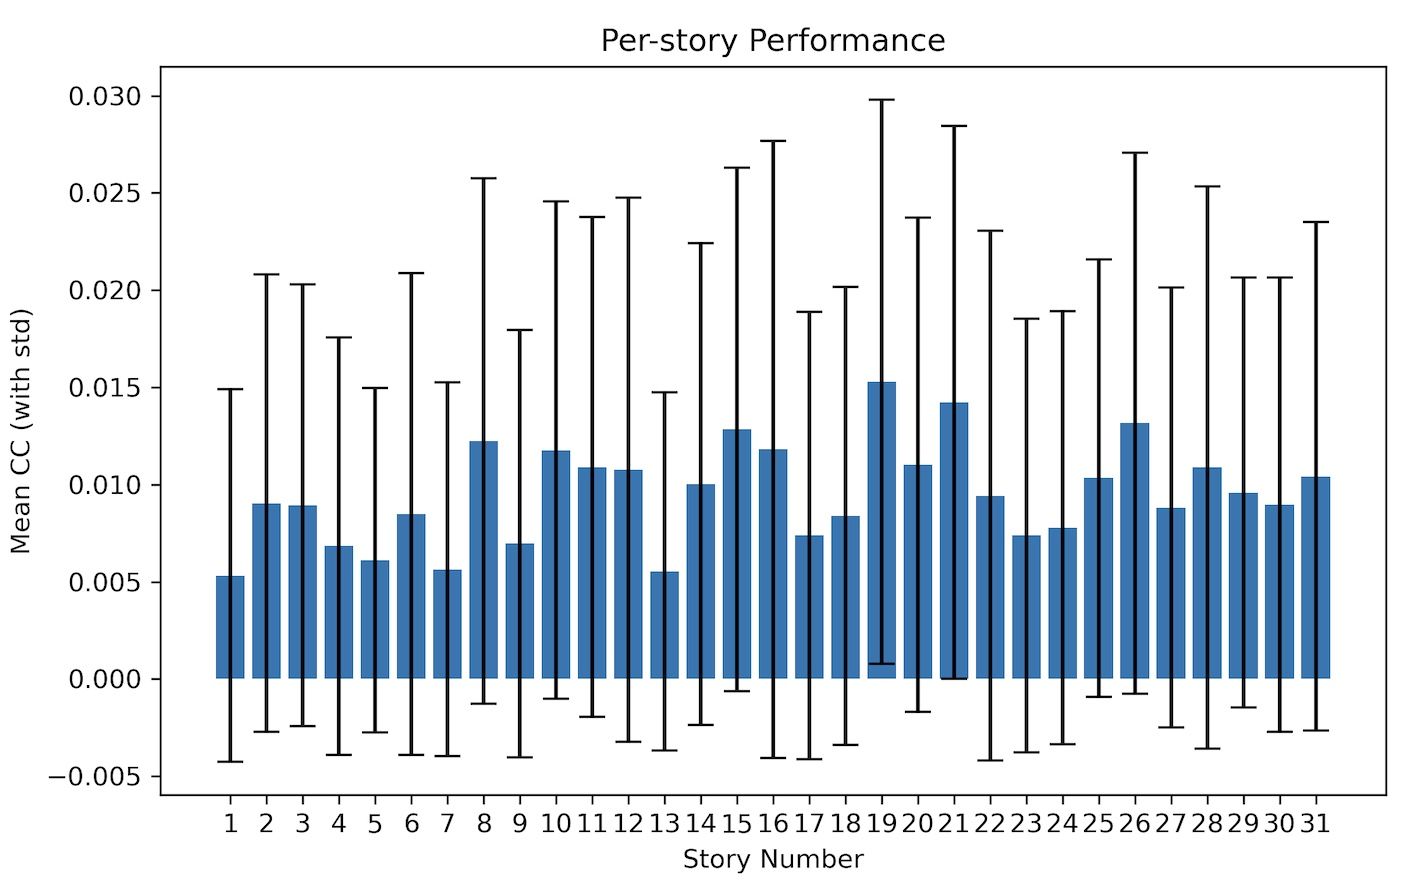
\includegraphics[width=\textwidth]{subject2_word2vec_stability.jpeg}
        \caption{Subject 2}
        \label{fig:word2vec_subject2_stability}
    \end{minipage}
    \hfill
    \begin{minipage}{0.45\textwidth}
        \centering
        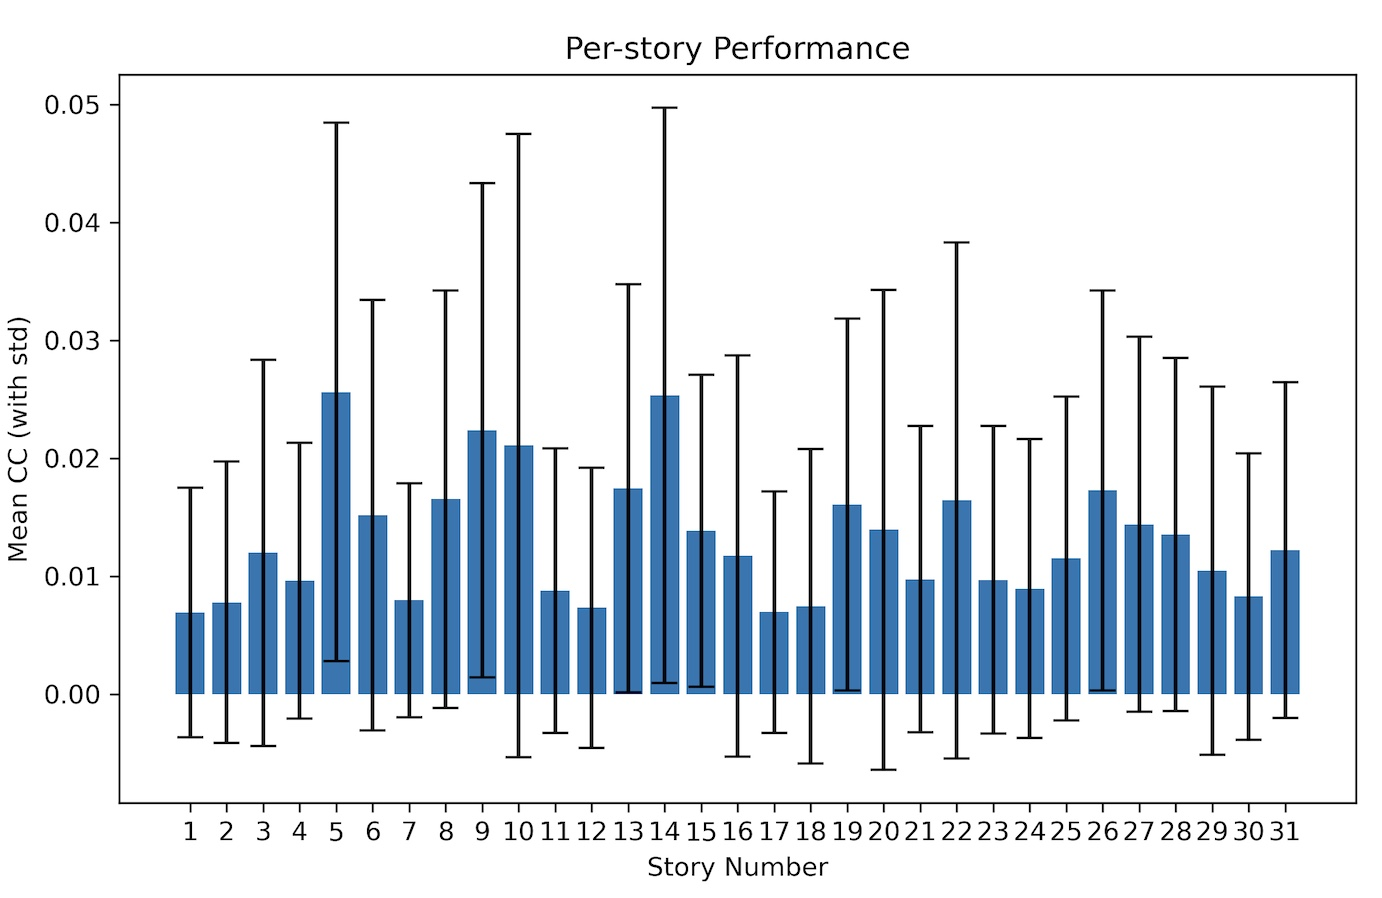
\includegraphics[width=\textwidth]{subject3_word2vec_stability.jpeg}
        \caption{Subject 3}
        \label{fig:word2vec_subject3_stability}
    \end{minipage}
    \caption{Word2Vec Performance across Test Stories}
    \label{fig:word2vec_stability}
\end{figure}


\section{Conclusion}
In summary, we have generated three types of word embeddings (Word2Vec, GloVe, BagOfWords) to obtain three sets of design matrices used for our ridge regression analysis. Due to computational constraints, the Word2Vec embedding required additional dimensionality reduction. Following this, we took the three embedding types and fitted ridge regression models for each voxel, cross validated on 3-fold cross validation to tune hyperparameter $\lambda$. 

In terms of our results, we identified that the Word2Vec embedding performed best out of our three embedding types. We then performed some post-hoc stability analysis to evaluate our results. Notably, we found that the Correlation Coefficient (CC) distribution for subject 2 and 3 were not significantly different and only a small number of voxels can be said to have a correlation overall and that even these voxels have a weak correlation. Additionally, we identified that highest-performing model for our highest-performing embedding type (Word2Vec) and corresponding ridge regression model, performed similarly across stories in the provided corpus.

The implication of our results indicates that we cannot confidently determine whether ridge regression and/or any of our embeddings (Word2Vec, GloVe, or BagOfWords) to be suitable for predicting the blood-oxygen level across voxels via fMRI brain scan data.  


\newpage

\section{Bibliography}

Jain, Shailee, and Alexander Huth. “Incorporating Context into Language Encoding Models for FMRI.” 

\section{Collaborators} 

I certify that I have only collaborated with my group members. 


\section{Academic honesty}
To: Bin Yu 

I declare that the work presented in Lab 3.1 is entirely my own and my group members. We ourself designed and performed all the data analysis, methods and procedures presented in this report. We ourself wrote all the texts, wrote codes embeddings, modeling, and produced all the figures in this report. We used codes provided by GSI. We have included and documented all the procedures in the workflow and the results are fully reproducible. Wherever we included the work from others, we cited the sources and in 'References section', especially for equations. We used LLM specifically for improved grammar for report writing style.

By submitting this lab report and all github material, I certify that we have complied with the academic integrity standards as set in lab 3.1 instructions. 

\section{References}

\begin{itemize}
    \item \href{https://medium.com/@manansuri/a-dummys-guide-to-word2vec-456444f3c673}{https://medium.com/@manansuri/a-dummys-guide-to-word2vec-456444f3c673}
    \item \href{https://en.wikipedia.org/wiki/Word2vec}{https://en.wikipedia.org/wiki/Word2vec}
    \item \href{https://en.wikipedia.org/wiki/GloVe}{https://en.wikipedia.org/wiki/GloVe}
    \item \href{https://paperswithcode.com/method/skip-gram-word2vec}{https://paperswithcode.com/method/skip-gram-word2vec}
    \item \href{https://becominghuman.ai/mathematical-introduction-to-glove-word-embedding-60f24154e54c}{https://becominghuman.ai/mathematical-introduction-to-glove-word-embedding-60f24154e54c}

    \item \href{https://www.sciencedirect.com/science/article/abs/pii/S0191886916308194}{https://www.sciencedirect.com/science/article/abs/pii/S0191886916308194}
    
    
\end{itemize}


\end{document}
